% Created by tikzDevice version 0.12.3.1 on 2021-04-21 15:16:41
% !TEX encoding = UTF-8 Unicode
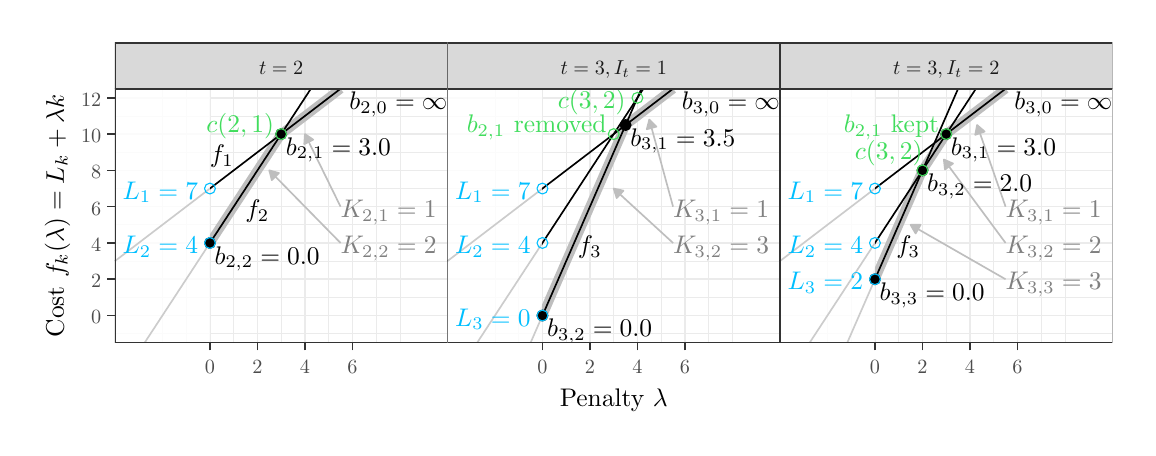
\begin{tikzpicture}[x=1pt,y=1pt]
\definecolor{fillColor}{RGB}{255,255,255}
\path[use as bounding box,fill=fillColor,fill opacity=0.00] (0,0) rectangle (397.48,144.54);
\begin{scope}
\path[clip] (  0.00,  0.00) rectangle (397.48,144.54);
\definecolor{drawColor}{RGB}{255,255,255}
\definecolor{fillColor}{RGB}{255,255,255}

\path[draw=drawColor,line width= 0.6pt,line join=round,line cap=round,fill=fillColor] (  0.00,  0.00) rectangle (397.48,144.54);
\end{scope}
\begin{scope}
\path[clip] ( 31.53, 30.69) rectangle (151.68,122.47);
\definecolor{fillColor}{RGB}{255,255,255}

\path[fill=fillColor] ( 31.53, 30.69) rectangle (151.68,122.47);
\definecolor{drawColor}{gray}{0.92}

\path[draw=drawColor,line width= 0.3pt,line join=round] ( 31.53, 33.96) --
	(151.68, 33.96);

\path[draw=drawColor,line width= 0.3pt,line join=round] ( 31.53, 47.08) --
	(151.68, 47.08);

\path[draw=drawColor,line width= 0.3pt,line join=round] ( 31.53, 60.19) --
	(151.68, 60.19);

\path[draw=drawColor,line width= 0.3pt,line join=round] ( 31.53, 73.30) --
	(151.68, 73.30);

\path[draw=drawColor,line width= 0.3pt,line join=round] ( 31.53, 86.41) --
	(151.68, 86.41);

\path[draw=drawColor,line width= 0.3pt,line join=round] ( 31.53, 99.52) --
	(151.68, 99.52);

\path[draw=drawColor,line width= 0.3pt,line join=round] ( 31.53,112.63) --
	(151.68,112.63);

\path[draw=drawColor,line width= 0.3pt,line join=round] ( 48.69, 30.69) --
	( 48.69,122.47);

\path[draw=drawColor,line width= 0.3pt,line join=round] ( 57.28, 30.69) --
	( 57.28,122.47);

\path[draw=drawColor,line width= 0.3pt,line join=round] ( 74.44, 30.69) --
	( 74.44,122.47);

\path[draw=drawColor,line width= 0.3pt,line join=round] ( 91.60, 30.69) --
	( 91.60,122.47);

\path[draw=drawColor,line width= 0.3pt,line join=round] (108.77, 30.69) --
	(108.77,122.47);

\path[draw=drawColor,line width= 0.3pt,line join=round] (125.93, 30.69) --
	(125.93,122.47);

\path[draw=drawColor,line width= 0.3pt,line join=round] (134.52, 30.69) --
	(134.52,122.47);

\path[draw=drawColor,line width= 0.6pt,line join=round] ( 31.53, 40.52) --
	(151.68, 40.52);

\path[draw=drawColor,line width= 0.6pt,line join=round] ( 31.53, 53.63) --
	(151.68, 53.63);

\path[draw=drawColor,line width= 0.6pt,line join=round] ( 31.53, 66.74) --
	(151.68, 66.74);

\path[draw=drawColor,line width= 0.6pt,line join=round] ( 31.53, 79.86) --
	(151.68, 79.86);

\path[draw=drawColor,line width= 0.6pt,line join=round] ( 31.53, 92.97) --
	(151.68, 92.97);

\path[draw=drawColor,line width= 0.6pt,line join=round] ( 31.53,106.08) --
	(151.68,106.08);

\path[draw=drawColor,line width= 0.6pt,line join=round] ( 31.53,119.19) --
	(151.68,119.19);

\path[draw=drawColor,line width= 0.6pt,line join=round] ( 65.86, 30.69) --
	( 65.86,122.47);

\path[draw=drawColor,line width= 0.6pt,line join=round] ( 83.02, 30.69) --
	( 83.02,122.47);

\path[draw=drawColor,line width= 0.6pt,line join=round] (100.19, 30.69) --
	(100.19,122.47);

\path[draw=drawColor,line width= 0.6pt,line join=round] (117.35, 30.69) --
	(117.35,122.47);
\definecolor{drawColor}{RGB}{190,190,190}

\path[draw=drawColor,line width= 3.4pt,line join=round] ( 65.86, 66.74) --
	( 66.72, 68.05) --
	( 67.57, 69.37) --
	( 68.43, 70.68) --
	( 69.29, 71.99) --
	( 70.15, 73.30) --
	( 71.01, 74.61) --
	( 71.87, 75.92) --
	( 72.72, 77.23) --
	( 73.58, 78.54) --
	( 74.44, 79.86) --
	( 75.30, 81.17) --
	( 76.16, 82.48) --
	( 77.02, 83.79) --
	( 77.87, 85.10) --
	( 78.73, 86.41) --
	( 79.59, 87.72) --
	( 80.45, 89.03) --
	( 81.31, 90.34) --
	( 82.16, 91.66) --
	( 83.02, 92.97) --
	( 83.88, 94.28) --
	( 84.74, 95.59) --
	( 85.60, 96.90) --
	( 86.46, 98.21) --
	( 87.31, 99.52) --
	( 88.17,100.83) --
	( 89.03,102.15) --
	( 89.89,103.46) --
	( 90.75,104.77) --
	( 91.60,106.08) --
	( 92.46,106.73) --
	( 93.32,107.39) --
	( 94.18,108.05) --
	( 95.04,108.70) --
	( 95.90,109.36) --
	( 96.75,110.01) --
	( 97.61,110.67) --
	( 98.47,111.32) --
	( 99.33,111.98) --
	(100.19,112.63) --
	(101.05,113.29) --
	(101.90,113.95) --
	(102.76,114.60) --
	(103.62,115.26) --
	(104.48,115.91) --
	(105.34,116.57) --
	(106.19,117.22) --
	(107.05,117.88) --
	(107.91,118.54) --
	(108.77,119.19) --
	(109.63,119.85) --
	(110.49,120.50) --
	(111.34,121.16) --
	(112.20,121.81) --
	(113.06,122.47);

\path[draw=drawColor,line width= 0.6pt,line join=round] (113.06, 79.86) -- (100.19,106.08);
\definecolor{fillColor}{RGB}{190,190,190}

\path[draw=drawColor,line width= 0.6pt,line join=round,fill=fillColor] (103.19,104.07) --
	(100.19,106.08) --
	( 99.94,102.47) --
	cycle;

\path[draw=drawColor,line width= 0.6pt,line join=round] (113.06, 66.74) -- ( 87.31, 92.97);

\path[draw=drawColor,line width= 0.6pt,line join=round,fill=fillColor] ( 90.80, 92.00) --
	( 87.31, 92.97) --
	( 88.22, 89.47) --
	cycle;
\definecolor{drawColor}{RGB}{0,0,0}

\node[text=drawColor,anchor=base west,inner sep=0pt, outer sep=0pt, scale=  0.92] at ( 67.57, 59.14) {$b_{2,2}=0.0$};

\node[text=drawColor,anchor=base west,inner sep=0pt, outer sep=0pt, scale=  0.92] at ( 93.32, 98.48) {$b_{2,1}=3.0$};

\path[draw=drawColor,line width= 0.6pt,line join=round] ( 31.53, 60.19) -- (141.95,144.54);

\path[draw=drawColor,line width= 0.6pt,line join=round] ( 31.53, 14.30) -- (116.78,144.54);
\definecolor{fillColor}{RGB}{255,255,255}

\path[fill=fillColor,fill opacity=0.80] ( 31.53, 30.69) rectangle ( 65.86,122.47);
\definecolor{drawColor}{gray}{0.50}

\node[text=drawColor,anchor=base west,inner sep=0pt, outer sep=0pt, scale=  0.92] at (113.06, 76.05) {$K_{2,1}=1$};

\node[text=drawColor,anchor=base west,inner sep=0pt, outer sep=0pt, scale=  0.92] at (113.06, 62.94) {$K_{2,2}=2$};
\definecolor{drawColor}{RGB}{0,0,0}
\definecolor{fillColor}{RGB}{0,0,0}

\path[draw=drawColor,line width= 0.4pt,line join=round,line cap=round,fill=fillColor] ( 65.86, 66.74) circle (  1.96);

\path[draw=drawColor,line width= 0.4pt,line join=round,line cap=round,fill=fillColor] ( 91.60,106.08) circle (  1.96);
\definecolor{drawColor}{RGB}{65,221,93}

\path[draw=drawColor,line width= 0.4pt,line join=round,line cap=round] ( 91.60,106.08) circle (  1.96);

\node[text=drawColor,anchor=base east,inner sep=0pt, outer sep=0pt, scale=  0.92] at ( 89.03,106.73) {$c(2, 1)$};
\definecolor{drawColor}{RGB}{0,0,0}

\node[text=drawColor,anchor=base,inner sep=0pt, outer sep=0pt, scale=  0.92] at ( 70.15, 95.72) {$f_1$};

\node[text=drawColor,anchor=base,inner sep=0pt, outer sep=0pt, scale=  0.92] at ( 83.02, 76.05) {$f_2$};

\node[text=drawColor,anchor=base east,inner sep=0pt, outer sep=0pt, scale=  0.92] at (151.68,114.87) {$b_{2,0}=\infty$};
\definecolor{drawColor}{RGB}{0,191,255}

\node[text=drawColor,anchor=base east,inner sep=0pt, outer sep=0pt, scale=  0.92] at ( 61.57, 82.61) {$L_1=7$};

\node[text=drawColor,anchor=base east,inner sep=0pt, outer sep=0pt, scale=  0.92] at ( 61.57, 62.94) {$L_2=4$};

\path[draw=drawColor,line width= 0.4pt,line join=round,line cap=round] ( 65.86, 86.41) circle (  1.96);

\path[draw=drawColor,line width= 0.4pt,line join=round,line cap=round] ( 65.86, 66.74) circle (  1.96);
\definecolor{drawColor}{gray}{0.20}

\path[draw=drawColor,line width= 0.6pt,line join=round,line cap=round] ( 31.53, 30.69) rectangle (151.68,122.47);
\end{scope}
\begin{scope}
\path[clip] (151.68, 30.69) rectangle (271.83,122.47);
\definecolor{fillColor}{RGB}{255,255,255}

\path[fill=fillColor] (151.68, 30.69) rectangle (271.83,122.47);
\definecolor{drawColor}{gray}{0.92}

\path[draw=drawColor,line width= 0.3pt,line join=round] (151.68, 33.96) --
	(271.83, 33.96);

\path[draw=drawColor,line width= 0.3pt,line join=round] (151.68, 47.08) --
	(271.83, 47.08);

\path[draw=drawColor,line width= 0.3pt,line join=round] (151.68, 60.19) --
	(271.83, 60.19);

\path[draw=drawColor,line width= 0.3pt,line join=round] (151.68, 73.30) --
	(271.83, 73.30);

\path[draw=drawColor,line width= 0.3pt,line join=round] (151.68, 86.41) --
	(271.83, 86.41);

\path[draw=drawColor,line width= 0.3pt,line join=round] (151.68, 99.52) --
	(271.83, 99.52);

\path[draw=drawColor,line width= 0.3pt,line join=round] (151.68,112.63) --
	(271.83,112.63);

\path[draw=drawColor,line width= 0.3pt,line join=round] (168.85, 30.69) --
	(168.85,122.47);

\path[draw=drawColor,line width= 0.3pt,line join=round] (177.43, 30.69) --
	(177.43,122.47);

\path[draw=drawColor,line width= 0.3pt,line join=round] (194.59, 30.69) --
	(194.59,122.47);

\path[draw=drawColor,line width= 0.3pt,line join=round] (211.76, 30.69) --
	(211.76,122.47);

\path[draw=drawColor,line width= 0.3pt,line join=round] (228.92, 30.69) --
	(228.92,122.47);

\path[draw=drawColor,line width= 0.3pt,line join=round] (246.09, 30.69) --
	(246.09,122.47);

\path[draw=drawColor,line width= 0.3pt,line join=round] (254.67, 30.69) --
	(254.67,122.47);

\path[draw=drawColor,line width= 0.6pt,line join=round] (151.68, 40.52) --
	(271.83, 40.52);

\path[draw=drawColor,line width= 0.6pt,line join=round] (151.68, 53.63) --
	(271.83, 53.63);

\path[draw=drawColor,line width= 0.6pt,line join=round] (151.68, 66.74) --
	(271.83, 66.74);

\path[draw=drawColor,line width= 0.6pt,line join=round] (151.68, 79.86) --
	(271.83, 79.86);

\path[draw=drawColor,line width= 0.6pt,line join=round] (151.68, 92.97) --
	(271.83, 92.97);

\path[draw=drawColor,line width= 0.6pt,line join=round] (151.68,106.08) --
	(271.83,106.08);

\path[draw=drawColor,line width= 0.6pt,line join=round] (151.68,119.19) --
	(271.83,119.19);

\path[draw=drawColor,line width= 0.6pt,line join=round] (186.01, 30.69) --
	(186.01,122.47);

\path[draw=drawColor,line width= 0.6pt,line join=round] (203.17, 30.69) --
	(203.17,122.47);

\path[draw=drawColor,line width= 0.6pt,line join=round] (220.34, 30.69) --
	(220.34,122.47);

\path[draw=drawColor,line width= 0.6pt,line join=round] (237.50, 30.69) --
	(237.50,122.47);
\definecolor{drawColor}{RGB}{190,190,190}

\path[draw=drawColor,line width= 3.4pt,line join=round] (186.01, 40.52) --
	(186.87, 42.49) --
	(187.73, 44.45) --
	(188.58, 46.42) --
	(189.44, 48.39) --
	(190.30, 50.35) --
	(191.16, 52.32) --
	(192.02, 54.29) --
	(192.88, 56.25) --
	(193.73, 58.22) --
	(194.59, 60.19) --
	(195.45, 62.15) --
	(196.31, 64.12) --
	(197.17, 66.09) --
	(198.03, 68.05) --
	(198.88, 70.02) --
	(199.74, 71.99) --
	(200.60, 73.95) --
	(201.46, 75.92) --
	(202.32, 77.89) --
	(203.17, 79.86) --
	(204.03, 81.82) --
	(204.89, 83.79) --
	(205.75, 85.76) --
	(206.61, 87.72) --
	(207.47, 89.69) --
	(208.32, 91.66) --
	(209.18, 93.62) --
	(210.04, 95.59) --
	(210.90, 97.56) --
	(211.76, 99.52) --
	(212.62,101.49) --
	(213.47,103.46) --
	(214.33,105.42) --
	(215.19,107.39) --
	(216.05,109.36) --
	(216.91,110.01) --
	(217.76,110.67) --
	(218.62,111.32) --
	(219.48,111.98) --
	(220.34,112.63) --
	(221.20,113.29) --
	(222.06,113.95) --
	(222.91,114.60) --
	(223.77,115.26) --
	(224.63,115.91) --
	(225.49,116.57) --
	(226.35,117.22) --
	(227.21,117.88) --
	(228.06,118.54) --
	(228.92,119.19) --
	(229.78,119.85) --
	(230.64,120.50) --
	(231.50,121.16) --
	(232.35,121.81) --
	(233.21,122.47);

\path[draw=drawColor,line width= 0.6pt,line join=round] (233.21, 79.86) -- (224.63,111.32);
\definecolor{fillColor}{RGB}{190,190,190}

\path[draw=drawColor,line width= 0.6pt,line join=round,fill=fillColor] (227.20,108.78) --
	(224.63,111.32) --
	(223.71,107.83) --
	cycle;

\path[draw=drawColor,line width= 0.6pt,line join=round] (233.21, 66.74) -- (211.76, 86.41);

\path[draw=drawColor,line width= 0.6pt,line join=round,fill=fillColor] (215.28, 85.63) --
	(211.76, 86.41) --
	(212.84, 82.96) --
	cycle;
\definecolor{drawColor}{RGB}{0,0,0}

\node[text=drawColor,anchor=base west,inner sep=0pt, outer sep=0pt, scale=  0.92] at (187.73, 32.92) {$b_{3,2}=0.0$};

\node[text=drawColor,anchor=base west,inner sep=0pt, outer sep=0pt, scale=  0.92] at (217.76,101.75) {$b_{3,1}=3.5$};

\path[draw=drawColor,line width= 0.6pt,line join=round] (151.68, 60.19) -- (262.11,144.54);

\path[draw=drawColor,line width= 0.6pt,line join=round] (151.68, 14.30) -- (236.93,144.54);

\path[draw=drawColor,line width= 0.6pt,line join=round] (168.33,  0.00) -- (231.40,144.54);
\definecolor{fillColor}{RGB}{255,255,255}

\path[fill=fillColor,fill opacity=0.80] (151.68, 30.69) rectangle (186.01,122.47);
\definecolor{drawColor}{gray}{0.50}

\node[text=drawColor,anchor=base west,inner sep=0pt, outer sep=0pt, scale=  0.92] at (233.21, 76.05) {$K_{3,1}=1$};

\node[text=drawColor,anchor=base west,inner sep=0pt, outer sep=0pt, scale=  0.92] at (233.21, 62.94) {$K_{3,2}=3$};
\definecolor{drawColor}{RGB}{0,0,0}
\definecolor{fillColor}{RGB}{0,0,0}

\path[draw=drawColor,line width= 0.4pt,line join=round,line cap=round,fill=fillColor] (186.01, 40.52) circle (  1.96);

\path[draw=drawColor,line width= 0.4pt,line join=round,line cap=round,fill=fillColor] (216.05,109.36) circle (  1.96);
\definecolor{drawColor}{RGB}{65,221,93}

\path[draw=drawColor,line width= 0.4pt,line join=round,line cap=round] (211.76,106.08) circle (  1.96);

\path[draw=drawColor,line width= 0.4pt,line join=round,line cap=round] (220.34,119.19) circle (  1.96);

\node[text=drawColor,anchor=base east,inner sep=0pt, outer sep=0pt, scale=  0.92] at (216.05,115.39) {$c(3, 2)$};

\node[text=drawColor,anchor=base east,inner sep=0pt, outer sep=0pt, scale=  0.92] at (209.18,106.73) {$b_{2,1}$ removed};
\definecolor{drawColor}{RGB}{0,0,0}

\node[text=drawColor,anchor=base,inner sep=0pt, outer sep=0pt, scale=  0.92] at (203.17, 62.94) {$f_3$};

\node[text=drawColor,anchor=base east,inner sep=0pt, outer sep=0pt, scale=  0.92] at (271.83,114.87) {$b_{3,0}=\infty$};
\definecolor{drawColor}{RGB}{0,191,255}

\node[text=drawColor,anchor=base east,inner sep=0pt, outer sep=0pt, scale=  0.92] at (181.72, 82.61) {$L_1=7$};

\node[text=drawColor,anchor=base east,inner sep=0pt, outer sep=0pt, scale=  0.92] at (181.72, 62.94) {$L_2=4$};

\node[text=drawColor,anchor=base east,inner sep=0pt, outer sep=0pt, scale=  0.92] at (181.72, 36.72) {$L_3=0$};

\path[draw=drawColor,line width= 0.4pt,line join=round,line cap=round] (186.01, 86.41) circle (  1.96);

\path[draw=drawColor,line width= 0.4pt,line join=round,line cap=round] (186.01, 66.74) circle (  1.96);

\path[draw=drawColor,line width= 0.4pt,line join=round,line cap=round] (186.01, 40.52) circle (  1.96);
\definecolor{drawColor}{gray}{0.20}

\path[draw=drawColor,line width= 0.6pt,line join=round,line cap=round] (151.68, 30.69) rectangle (271.83,122.47);
\end{scope}
\begin{scope}
\path[clip] (271.83, 30.69) rectangle (391.98,122.47);
\definecolor{fillColor}{RGB}{255,255,255}

\path[fill=fillColor] (271.83, 30.69) rectangle (391.98,122.47);
\definecolor{drawColor}{gray}{0.92}

\path[draw=drawColor,line width= 0.3pt,line join=round] (271.83, 33.96) --
	(391.98, 33.96);

\path[draw=drawColor,line width= 0.3pt,line join=round] (271.83, 47.08) --
	(391.98, 47.08);

\path[draw=drawColor,line width= 0.3pt,line join=round] (271.83, 60.19) --
	(391.98, 60.19);

\path[draw=drawColor,line width= 0.3pt,line join=round] (271.83, 73.30) --
	(391.98, 73.30);

\path[draw=drawColor,line width= 0.3pt,line join=round] (271.83, 86.41) --
	(391.98, 86.41);

\path[draw=drawColor,line width= 0.3pt,line join=round] (271.83, 99.52) --
	(391.98, 99.52);

\path[draw=drawColor,line width= 0.3pt,line join=round] (271.83,112.63) --
	(391.98,112.63);

\path[draw=drawColor,line width= 0.3pt,line join=round] (289.00, 30.69) --
	(289.00,122.47);

\path[draw=drawColor,line width= 0.3pt,line join=round] (297.58, 30.69) --
	(297.58,122.47);

\path[draw=drawColor,line width= 0.3pt,line join=round] (314.74, 30.69) --
	(314.74,122.47);

\path[draw=drawColor,line width= 0.3pt,line join=round] (331.91, 30.69) --
	(331.91,122.47);

\path[draw=drawColor,line width= 0.3pt,line join=round] (349.07, 30.69) --
	(349.07,122.47);

\path[draw=drawColor,line width= 0.3pt,line join=round] (366.24, 30.69) --
	(366.24,122.47);

\path[draw=drawColor,line width= 0.3pt,line join=round] (374.82, 30.69) --
	(374.82,122.47);

\path[draw=drawColor,line width= 0.6pt,line join=round] (271.83, 40.52) --
	(391.98, 40.52);

\path[draw=drawColor,line width= 0.6pt,line join=round] (271.83, 53.63) --
	(391.98, 53.63);

\path[draw=drawColor,line width= 0.6pt,line join=round] (271.83, 66.74) --
	(391.98, 66.74);

\path[draw=drawColor,line width= 0.6pt,line join=round] (271.83, 79.86) --
	(391.98, 79.86);

\path[draw=drawColor,line width= 0.6pt,line join=round] (271.83, 92.97) --
	(391.98, 92.97);

\path[draw=drawColor,line width= 0.6pt,line join=round] (271.83,106.08) --
	(391.98,106.08);

\path[draw=drawColor,line width= 0.6pt,line join=round] (271.83,119.19) --
	(391.98,119.19);

\path[draw=drawColor,line width= 0.6pt,line join=round] (306.16, 30.69) --
	(306.16,122.47);

\path[draw=drawColor,line width= 0.6pt,line join=round] (323.33, 30.69) --
	(323.33,122.47);

\path[draw=drawColor,line width= 0.6pt,line join=round] (340.49, 30.69) --
	(340.49,122.47);

\path[draw=drawColor,line width= 0.6pt,line join=round] (357.66, 30.69) --
	(357.66,122.47);
\definecolor{drawColor}{RGB}{190,190,190}

\path[draw=drawColor,line width= 3.4pt,line join=round] (306.16, 53.63) --
	(307.02, 55.60) --
	(307.88, 57.57) --
	(308.74, 59.53) --
	(309.60, 61.50) --
	(310.45, 63.47) --
	(311.31, 65.43) --
	(312.17, 67.40) --
	(313.03, 69.37) --
	(313.89, 71.33) --
	(314.74, 73.30) --
	(315.60, 75.27) --
	(316.46, 77.23) --
	(317.32, 79.20) --
	(318.18, 81.17) --
	(319.04, 83.13) --
	(319.89, 85.10) --
	(320.75, 87.07) --
	(321.61, 89.03) --
	(322.47, 91.00) --
	(323.33, 92.97) --
	(324.18, 94.28) --
	(325.04, 95.59) --
	(325.90, 96.90) --
	(326.76, 98.21) --
	(327.62, 99.52) --
	(328.48,100.83) --
	(329.33,102.15) --
	(330.19,103.46) --
	(331.05,104.77) --
	(331.91,106.08) --
	(332.77,106.73) --
	(333.63,107.39) --
	(334.48,108.05) --
	(335.34,108.70) --
	(336.20,109.36) --
	(337.06,110.01) --
	(337.92,110.67) --
	(338.77,111.32) --
	(339.63,111.98) --
	(340.49,112.63) --
	(341.35,113.29) --
	(342.21,113.95) --
	(343.07,114.60) --
	(343.92,115.26) --
	(344.78,115.91) --
	(345.64,116.57) --
	(346.50,117.22) --
	(347.36,117.88) --
	(348.22,118.54) --
	(349.07,119.19) --
	(349.93,119.85) --
	(350.79,120.50) --
	(351.65,121.16) --
	(352.51,121.81) --
	(353.36,122.47);

\path[draw=drawColor,line width= 0.6pt,line join=round] (353.36, 79.86) -- (343.07,109.36);
\definecolor{fillColor}{RGB}{190,190,190}

\path[draw=drawColor,line width= 0.6pt,line join=round,fill=fillColor] (345.80,107.00) --
	(343.07,109.36) --
	(342.39,105.81) --
	cycle;

\path[draw=drawColor,line width= 0.6pt,line join=round] (353.36, 66.74) -- (331.05, 96.90);

\path[draw=drawColor,line width= 0.6pt,line join=round,fill=fillColor] (334.36, 95.46) --
	(331.05, 96.90) --
	(331.46, 93.31) --
	cycle;

\path[draw=drawColor,line width= 0.6pt,line join=round] (353.36, 53.63) -- (319.04, 73.30);

\path[draw=drawColor,line width= 0.6pt,line join=round,fill=fillColor] (322.65, 73.31) --
	(319.04, 73.30) --
	(320.85, 70.18) --
	cycle;
\definecolor{drawColor}{RGB}{0,0,0}

\node[text=drawColor,anchor=base west,inner sep=0pt, outer sep=0pt, scale=  0.92] at (307.88, 46.03) {$b_{3,3}=0.0$};

\node[text=drawColor,anchor=base west,inner sep=0pt, outer sep=0pt, scale=  0.92] at (325.04, 85.36) {$b_{3,2}=2.0$};

\node[text=drawColor,anchor=base west,inner sep=0pt, outer sep=0pt, scale=  0.92] at (333.63, 98.48) {$b_{3,1}=3.0$};

\path[draw=drawColor,line width= 0.6pt,line join=round] (271.83, 60.19) -- (382.26,144.54);

\path[draw=drawColor,line width= 0.6pt,line join=round] (271.83, 14.30) -- (357.08,144.54);

\path[draw=drawColor,line width= 0.6pt,line join=round] (282.76,  0.00) -- (345.83,144.54);
\definecolor{fillColor}{RGB}{255,255,255}

\path[fill=fillColor,fill opacity=0.80] (271.83, 30.69) rectangle (306.16,122.47);
\definecolor{drawColor}{gray}{0.50}

\node[text=drawColor,anchor=base west,inner sep=0pt, outer sep=0pt, scale=  0.92] at (353.36, 76.05) {$K_{3,1}=1$};

\node[text=drawColor,anchor=base west,inner sep=0pt, outer sep=0pt, scale=  0.92] at (353.36, 62.94) {$K_{3,2}=2$};

\node[text=drawColor,anchor=base west,inner sep=0pt, outer sep=0pt, scale=  0.92] at (353.36, 49.83) {$K_{3,3}=3$};
\definecolor{drawColor}{RGB}{0,0,0}
\definecolor{fillColor}{RGB}{0,0,0}

\path[draw=drawColor,line width= 0.4pt,line join=round,line cap=round,fill=fillColor] (306.16, 53.63) circle (  1.96);

\path[draw=drawColor,line width= 0.4pt,line join=round,line cap=round,fill=fillColor] (323.33, 92.97) circle (  1.96);

\path[draw=drawColor,line width= 0.4pt,line join=round,line cap=round,fill=fillColor] (331.91,106.08) circle (  1.96);
\definecolor{drawColor}{RGB}{65,221,93}

\path[draw=drawColor,line width= 0.4pt,line join=round,line cap=round] (331.91,106.08) circle (  1.96);

\path[draw=drawColor,line width= 0.4pt,line join=round,line cap=round] (323.33, 92.97) circle (  1.96);

\node[text=drawColor,anchor=base east,inner sep=0pt, outer sep=0pt, scale=  0.92] at (323.33, 96.77) {$c(3, 2)$};

\node[text=drawColor,anchor=base east,inner sep=0pt, outer sep=0pt, scale=  0.92] at (329.33,106.73) {$b_{2,1}$ kept};
\definecolor{drawColor}{RGB}{0,0,0}

\node[text=drawColor,anchor=base,inner sep=0pt, outer sep=0pt, scale=  0.92] at (318.18, 62.94) {$f_3$};

\node[text=drawColor,anchor=base east,inner sep=0pt, outer sep=0pt, scale=  0.92] at (391.98,114.87) {$b_{3,0}=\infty$};
\definecolor{drawColor}{RGB}{0,191,255}

\node[text=drawColor,anchor=base east,inner sep=0pt, outer sep=0pt, scale=  0.92] at (301.87, 82.61) {$L_1=7$};

\node[text=drawColor,anchor=base east,inner sep=0pt, outer sep=0pt, scale=  0.92] at (301.87, 62.94) {$L_2=4$};

\node[text=drawColor,anchor=base east,inner sep=0pt, outer sep=0pt, scale=  0.92] at (301.87, 49.83) {$L_3=2$};

\path[draw=drawColor,line width= 0.4pt,line join=round,line cap=round] (306.16, 86.41) circle (  1.96);

\path[draw=drawColor,line width= 0.4pt,line join=round,line cap=round] (306.16, 66.74) circle (  1.96);

\path[draw=drawColor,line width= 0.4pt,line join=round,line cap=round] (306.16, 53.63) circle (  1.96);
\definecolor{drawColor}{gray}{0.20}

\path[draw=drawColor,line width= 0.6pt,line join=round,line cap=round] (271.83, 30.69) rectangle (391.98,122.47);
\end{scope}
\begin{scope}
\path[clip] ( 31.53,122.47) rectangle (151.68,139.04);
\definecolor{drawColor}{gray}{0.20}
\definecolor{fillColor}{gray}{0.85}

\path[draw=drawColor,line width= 0.6pt,line join=round,line cap=round,fill=fillColor] ( 31.53,122.47) rectangle (151.68,139.04);
\definecolor{drawColor}{gray}{0.10}

\node[text=drawColor,anchor=base,inner sep=0pt, outer sep=0pt, scale=  0.73] at ( 91.60,127.72) {$t=2$};
\end{scope}
\begin{scope}
\path[clip] (151.68,122.47) rectangle (271.83,139.04);
\definecolor{drawColor}{gray}{0.20}
\definecolor{fillColor}{gray}{0.85}

\path[draw=drawColor,line width= 0.6pt,line join=round,line cap=round,fill=fillColor] (151.68,122.47) rectangle (271.83,139.04);
\definecolor{drawColor}{gray}{0.10}

\node[text=drawColor,anchor=base,inner sep=0pt, outer sep=0pt, scale=  0.73] at (211.76,127.72) {$t=3, I_t=1$};
\end{scope}
\begin{scope}
\path[clip] (271.83,122.47) rectangle (391.98,139.04);
\definecolor{drawColor}{gray}{0.20}
\definecolor{fillColor}{gray}{0.85}

\path[draw=drawColor,line width= 0.6pt,line join=round,line cap=round,fill=fillColor] (271.83,122.47) rectangle (391.98,139.04);
\definecolor{drawColor}{gray}{0.10}

\node[text=drawColor,anchor=base,inner sep=0pt, outer sep=0pt, scale=  0.73] at (331.91,127.72) {$t=3, I_t=2$};
\end{scope}
\begin{scope}
\path[clip] (  0.00,  0.00) rectangle (397.48,144.54);
\definecolor{drawColor}{gray}{0.20}

\path[draw=drawColor,line width= 0.6pt,line join=round] ( 65.86, 27.94) --
	( 65.86, 30.69);

\path[draw=drawColor,line width= 0.6pt,line join=round] ( 83.02, 27.94) --
	( 83.02, 30.69);

\path[draw=drawColor,line width= 0.6pt,line join=round] (100.19, 27.94) --
	(100.19, 30.69);

\path[draw=drawColor,line width= 0.6pt,line join=round] (117.35, 27.94) --
	(117.35, 30.69);
\end{scope}
\begin{scope}
\path[clip] (  0.00,  0.00) rectangle (397.48,144.54);
\definecolor{drawColor}{gray}{0.30}

\node[text=drawColor,anchor=base,inner sep=0pt, outer sep=0pt, scale=  0.73] at ( 65.86, 19.68) {0};

\node[text=drawColor,anchor=base,inner sep=0pt, outer sep=0pt, scale=  0.73] at ( 83.02, 19.68) {2};

\node[text=drawColor,anchor=base,inner sep=0pt, outer sep=0pt, scale=  0.73] at (100.19, 19.68) {4};

\node[text=drawColor,anchor=base,inner sep=0pt, outer sep=0pt, scale=  0.73] at (117.35, 19.68) {6};
\end{scope}
\begin{scope}
\path[clip] (  0.00,  0.00) rectangle (397.48,144.54);
\definecolor{drawColor}{gray}{0.20}

\path[draw=drawColor,line width= 0.6pt,line join=round] (186.01, 27.94) --
	(186.01, 30.69);

\path[draw=drawColor,line width= 0.6pt,line join=round] (203.17, 27.94) --
	(203.17, 30.69);

\path[draw=drawColor,line width= 0.6pt,line join=round] (220.34, 27.94) --
	(220.34, 30.69);

\path[draw=drawColor,line width= 0.6pt,line join=round] (237.50, 27.94) --
	(237.50, 30.69);
\end{scope}
\begin{scope}
\path[clip] (  0.00,  0.00) rectangle (397.48,144.54);
\definecolor{drawColor}{gray}{0.30}

\node[text=drawColor,anchor=base,inner sep=0pt, outer sep=0pt, scale=  0.73] at (186.01, 19.68) {0};

\node[text=drawColor,anchor=base,inner sep=0pt, outer sep=0pt, scale=  0.73] at (203.17, 19.68) {2};

\node[text=drawColor,anchor=base,inner sep=0pt, outer sep=0pt, scale=  0.73] at (220.34, 19.68) {4};

\node[text=drawColor,anchor=base,inner sep=0pt, outer sep=0pt, scale=  0.73] at (237.50, 19.68) {6};
\end{scope}
\begin{scope}
\path[clip] (  0.00,  0.00) rectangle (397.48,144.54);
\definecolor{drawColor}{gray}{0.20}

\path[draw=drawColor,line width= 0.6pt,line join=round] (306.16, 27.94) --
	(306.16, 30.69);

\path[draw=drawColor,line width= 0.6pt,line join=round] (323.33, 27.94) --
	(323.33, 30.69);

\path[draw=drawColor,line width= 0.6pt,line join=round] (340.49, 27.94) --
	(340.49, 30.69);

\path[draw=drawColor,line width= 0.6pt,line join=round] (357.66, 27.94) --
	(357.66, 30.69);
\end{scope}
\begin{scope}
\path[clip] (  0.00,  0.00) rectangle (397.48,144.54);
\definecolor{drawColor}{gray}{0.30}

\node[text=drawColor,anchor=base,inner sep=0pt, outer sep=0pt, scale=  0.73] at (306.16, 19.68) {0};

\node[text=drawColor,anchor=base,inner sep=0pt, outer sep=0pt, scale=  0.73] at (323.33, 19.68) {2};

\node[text=drawColor,anchor=base,inner sep=0pt, outer sep=0pt, scale=  0.73] at (340.49, 19.68) {4};

\node[text=drawColor,anchor=base,inner sep=0pt, outer sep=0pt, scale=  0.73] at (357.66, 19.68) {6};
\end{scope}
\begin{scope}
\path[clip] (  0.00,  0.00) rectangle (397.48,144.54);
\definecolor{drawColor}{gray}{0.30}

\node[text=drawColor,anchor=base east,inner sep=0pt, outer sep=0pt, scale=  0.73] at ( 26.58, 37.49) {0};

\node[text=drawColor,anchor=base east,inner sep=0pt, outer sep=0pt, scale=  0.73] at ( 26.58, 50.60) {2};

\node[text=drawColor,anchor=base east,inner sep=0pt, outer sep=0pt, scale=  0.73] at ( 26.58, 63.71) {4};

\node[text=drawColor,anchor=base east,inner sep=0pt, outer sep=0pt, scale=  0.73] at ( 26.58, 76.83) {6};

\node[text=drawColor,anchor=base east,inner sep=0pt, outer sep=0pt, scale=  0.73] at ( 26.58, 89.94) {8};

\node[text=drawColor,anchor=base east,inner sep=0pt, outer sep=0pt, scale=  0.73] at ( 26.58,103.05) {10};

\node[text=drawColor,anchor=base east,inner sep=0pt, outer sep=0pt, scale=  0.73] at ( 26.58,116.16) {12};
\end{scope}
\begin{scope}
\path[clip] (  0.00,  0.00) rectangle (397.48,144.54);
\definecolor{drawColor}{gray}{0.20}

\path[draw=drawColor,line width= 0.6pt,line join=round] ( 28.78, 40.52) --
	( 31.53, 40.52);

\path[draw=drawColor,line width= 0.6pt,line join=round] ( 28.78, 53.63) --
	( 31.53, 53.63);

\path[draw=drawColor,line width= 0.6pt,line join=round] ( 28.78, 66.74) --
	( 31.53, 66.74);

\path[draw=drawColor,line width= 0.6pt,line join=round] ( 28.78, 79.86) --
	( 31.53, 79.86);

\path[draw=drawColor,line width= 0.6pt,line join=round] ( 28.78, 92.97) --
	( 31.53, 92.97);

\path[draw=drawColor,line width= 0.6pt,line join=round] ( 28.78,106.08) --
	( 31.53,106.08);

\path[draw=drawColor,line width= 0.6pt,line join=round] ( 28.78,119.19) --
	( 31.53,119.19);
\end{scope}
\begin{scope}
\path[clip] (  0.00,  0.00) rectangle (397.48,144.54);
\definecolor{drawColor}{RGB}{0,0,0}

\node[text=drawColor,anchor=base,inner sep=0pt, outer sep=0pt, scale=  0.92] at (211.76,  7.64) {Penalty $\lambda$};
\end{scope}
\begin{scope}
\path[clip] (  0.00,  0.00) rectangle (397.48,144.54);
\definecolor{drawColor}{RGB}{0,0,0}

\node[text=drawColor,rotate= 90.00,anchor=base,inner sep=0pt, outer sep=0pt, scale=  0.92] at ( 13.08, 76.58) {Cost $f_k(\lambda) = L_k + \lambda k$};
\end{scope}
\end{tikzpicture}
